\chapter{Teoria das Probabilidades}
\section{Introdução}

\inic A teoria dos conjuntos é a parte da matemática que trata das propriedades dos conjuntos, tendo sua origem nos trabalhos do matemático \textbf{Georg Ferdinand Ludwig Philipp Cantor(1845-1918)}, e se baseia na idéia de definir conjunto como uma noção primitiva. Algumas Vezes chamada de teoria ingênua ou intuitiva devido a descoberta de vários antinomias (ou paradoxos) relacionados a definição de conjunto.\vskip0.3cm

\inic Estas antinomias na teoria dos conjuntos conduziram a matemática a \textbf{Axiomatizar} as teorias  matemáticas, com influências profundas sobre a lógica e os fundamentos da matemática.


\begin{figure}
    \centering
    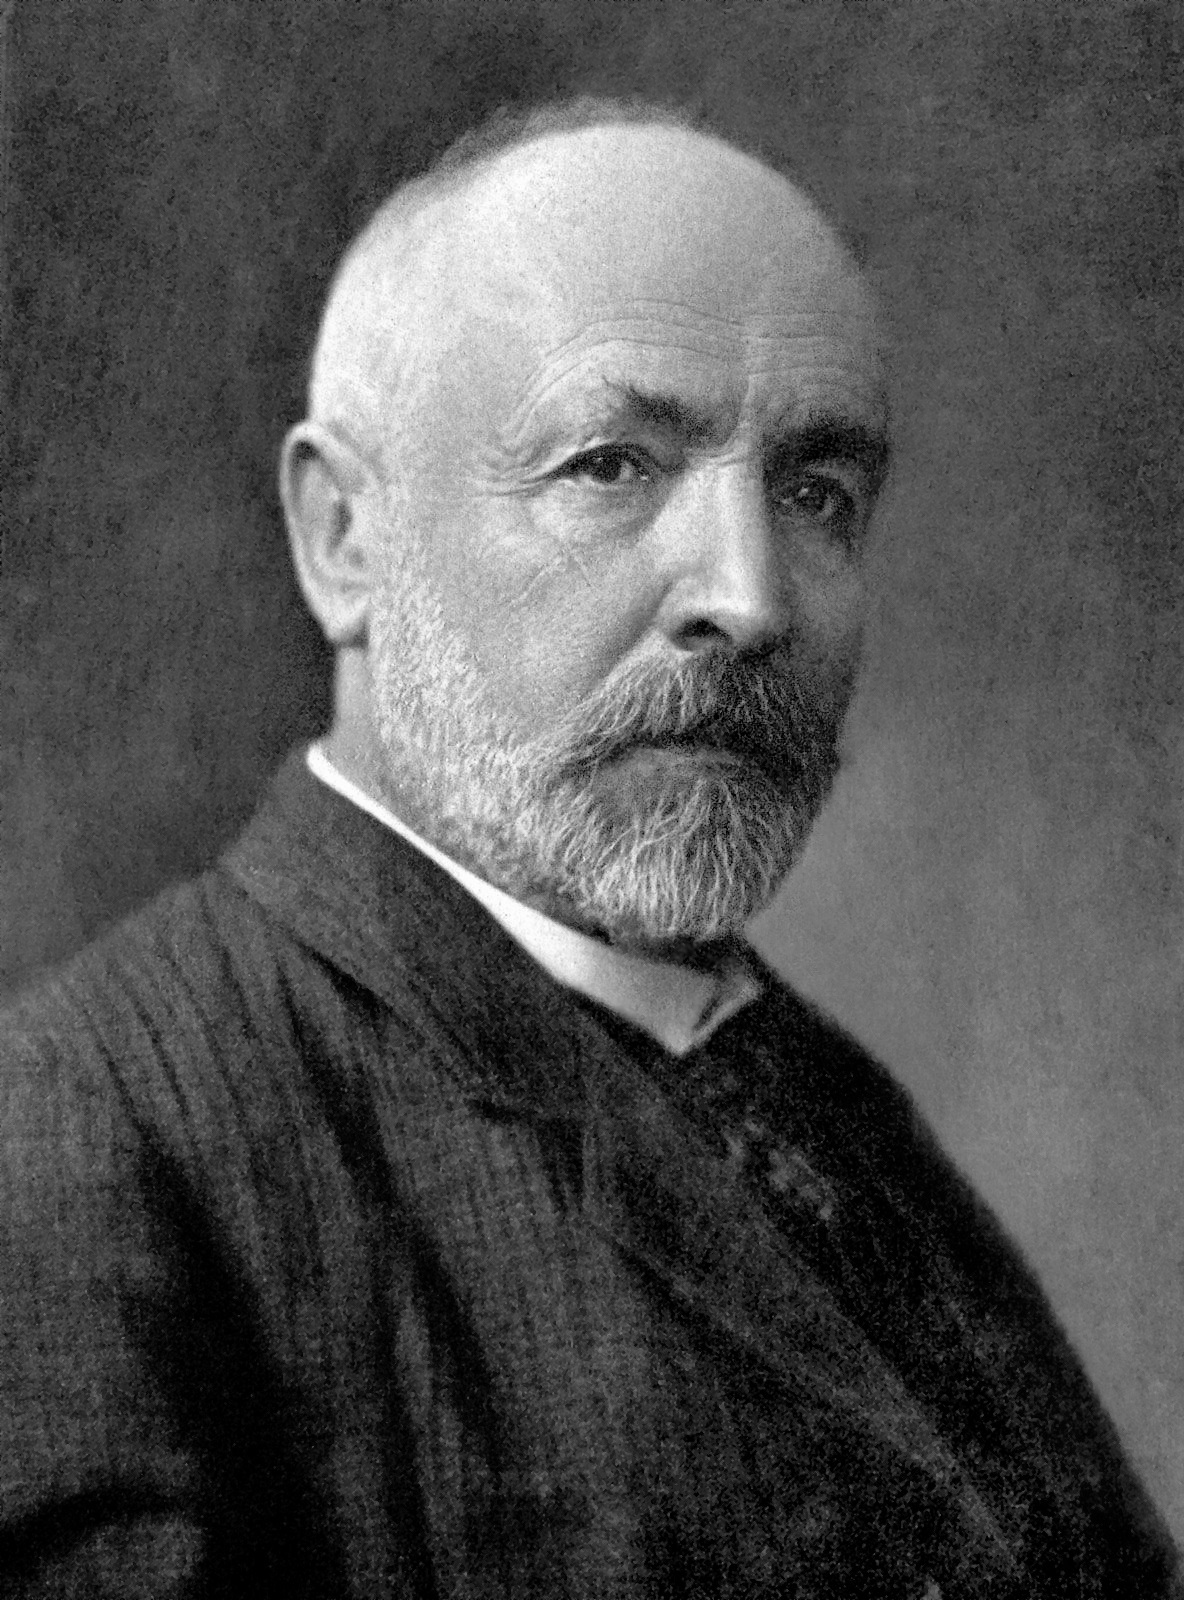
\includegraphics[scale=0.1]{figures/Cantor1.jpeg}
    \caption{Georg Ferdinand
Ludwig Philipp Cantor(1845-1918)}
    \label{fig:my_label}
\end{figure}



\inic A teoria teve seu início com a publicação em 1874 de um trabalho de Cantor que tratava sobre a comparação de coleções infinitas. Cantor, nasceu em São Petersburgo (Rússia), filho do comerciante dinamarquês, George Waldemar Cantor, e de uma musicista russa, Maria Anna Böhm. Em 1856 sua família mudou-se para a Alemanha, continuando aí os seus estudos. Estudou no Instituto Federal de Tecnologia de Zurique. Doutorou-se na Universidade de Berlim em 1867.\vskip0.3cm

\inic Desde 1638, com \textbf{Galileu Galilei}, sabe-se que se pode obter uma correspondência 1-1 entre os números inteiros e seus quadrados, o que violava a concepçao euclidiana de que o todo é sempre maior que qualquer uam de suas partes.\vskip0.3cm

\inic Esta aplicação de correspondência 1-1 permitiu a Cantor introduzir um método de diagnalização, que por contradição, permita provar que o conjunto dos números reais não tinha correspondência 1-1 com o conjunto dos números inteiros. Isto, mais tarde, levou ao desenvolvimento do conceito de contínuo por \textbf{Richard Dedekind}. \vskip0.3cm

\inic Em meados de 1892, Cantor, provou que o conjunto dos números racionais $Q$ é (e)numerável, enquanto que o conjunto dos números reais $IR$ é contínuo (logo, maior que o anterior). Já em 1897, Cantor descobriu vários paradoxos suscitados pela teoria dos conjuntos. Foi ele que utilizou pela primeira vez o símbolo ${\displaystyle \mathbb {R}}$ para representar o conjunto dos números reais.\vskip0.3cm


\inic Iniciando com estas descobertas, Cantor acabou desenvolvendo uma \textbf{Teoria dos Conjuntos} abstratos, que constitui-se em uma generalização do conceito de conjunto usada até hoje em vários ramos de pesquisa. \vskip0.3cm


Perseguido e criticado por sua tese, teve a saúde mental comprometida. Tempos depois, seus métodos foram assimilados e se mostraram perfeitamente práticos e úteis. Reconhecido alguns anos depois, foi nomeado membro honorário da \textbf{London Mathematical Society} e homenageado com a medalha da \textbf{Royal Society of London}.\vskip0.3cm

%Perturbado pelas perseguições, morreu aos 72 anos, em uma clínica psiquiátrica na Alemanha.



\section{Conjuntos}

O conceito de conjunto é fundamental não somente no estudo da
Probabilidade e da Estatística, como para a Matemática em geral.
\emph{Qualquer lista ou coleção bem definida de entidades ou
objetos é chamada conjunto}, os objetos que individualmente formam
ou compõem a coleção ou conjunto são chamados \emph{elementos ou
membros}. Em geral, denota-se um conjunto por uma letra maiúscula
($A,B,C,...$) e um elemento do conjunto por letra minúscula
($a,b,c,...$).\vskip0.3cm

\section{Subconjuntos}

Se todo elemento de um conjunto A é também elemento de um conjunto
B, dizemos que A é subconjunto de B, e escrevemos $A \subset B $
ou $B \supset A$ e lemos "A está contido em B", ou "B contém
A".\vskip0.3cm

Se um elemento $a$ pertence a um conjunto $C$ escrevemos $a \in
C$. Se $a$ não pertence a $C$ escrevemos $a \in C$. Se tanto $a$
como $b$ pertencem a $C$ escrevemos $a,b \in C$. A fim de que um
conjunto seja bem definido, devemos dispor de uma regra que nos
permita dizer se determinado objeto pertence ou não ao
conjunto.\vskip0.3cm

Um conjunto pode ser definido relacionando-se todos os seus
elementos, ou, quando isto não for possível, indicando uma
propriedade que seja válida para todos os elementos do conjunto, e
somente para eles.\vskip0.3cm


Existem três meneiras de descrever que objetos estão contidos no
conjunto A.

\begin{enumerate}
    \item Poderemos fazer uma lista dos elementos de A. Por
    exemplo, $A = \{ 1,2,3,4 \}$ descreve o conjunto formado pelos
    inteiros positivos 1,2,3 e 4.
    \item Poderemos descrever o conjunto A por meio de palavras.
    Por exemplo, poderemos dizer que A é formado de todos os
    números reais entre 0 e 1, inclusive.
    \item Para descrever o conjunto acima poderemos simplesmente
    escrever $A = \{ x|0\leq x \leq 1 \}$; isto é, A é o conjunto
    de todos os x, onde x é um número real entre 0 e 1, inclusive.
\end{enumerate}


\section{Experimentos Aleatórios}

È aquele que repetido em condições idênticas produz geralmente
resultados distintos. Por exemplo jogar uma moeda não viciada,
sabemos que a chance de sair cara é 50\%, mas não conseguimos
prever com exatidão o resultado da jogada, mesmo controlando todas
as circunstâncias relevantes ao experimento.\vskip0.3cm


\textbf{Ex1}: Lançar uma moeda três vezes. \vskip0.3cm

\textbf{Ex2}: Lançar dois dados simultaneamente. \vskip0.3cm

%\newpage
\subsection{Características dos Experimentos Aleatórios}

%Observando-se os experimentos acima pode-se destacar algumas
%características comuns.

\begin{itemize}
    \item Podem ser repetidos indefinidamente sob as mesmas
   condições;
   \item Não se pode adiantar um resultado particular, mas
    pode-se descrever todos os resultados possíveis;
    \item Se repetidos muitas vezes apresentarão uma regularidade
    em termos de frequências de resultados.
\end{itemize}


\section{Fenômenos Aleatórios}

O conceito de fenômeno aleatório é ligeiramente diferente do
conceito de experimento aleatório. Nos experimentos aleatórios
podemos controlar, de certa forma, fatores alheios ao problema os
quais podem influenciar os resultados do experimento, além disso,
podemos "reproduzir" o experimento com certa margem de
liberdade.\vskip0.3cm

Já nos fenômenos aleatórios nós somos meros observadores, os
fenômenos aleatórios tratados pela estatística são aqueles que
possuem "regularidade estatística", isto é, são observáveis e
suceptíveis de repetição.\vskip0.3cm

\textbf{Ex1}: Observar o número de casos de Meningite por mês em
Belém. \vskip0.3cm

\textbf{Ex2}: Observar a quantidade de chuva mensal.\vskip0.3cm



\section{Espaço Amostral ($\Omega$)}

Em um fenômeno aleatório ou probabilístico, isto é, sujeito às
leis do acaso, chamamos \emph{espaço amostral} ou \emph{espaço das
possibilidades} ao conjunto (em geral o mais detalhado possível)
de todos os resultados possíveis de ocorrer. Denota-lo-emos por
$S$ ou $\Omega$.\vskip0.3cm

Por exemplo, se jogarmos um dado vermelho e um dado preto, o
espaço amostral correspondente poderá ser descrito como segue.

$$
S_{1} =
\left[%
\begin{array}{cccccc}
  (1,1) & (2,1) & (3,1) & (4,1) & (5,1) & (6,1) \\
  (1,2) & (2,2) & (3,2) & (4,2) & (5,2) & (6,2) \\
  (1,3) & (2,3) & (3,3) & (4,3) & (5,3) & (6,3) \\
  (1,4) & (2,4) & (3,4) & (4,4) & (5,4) & (6,4) \\
  (1,5) & (2,5) & (3,5) & (4,5) & (5,5) & (6,5) \\
  (1,6) & (2,6) & (3,6) & (4,6) & (5,6) & (6,6) \\
\end{array}%
\right]
$$

Onde, digamos, o primeiro número de cada par indica o ponto do
dado branco e o segundo indica o ponto do dado preto. Entretanto, deve-se notar que, mesmo que os dados fossem
idênticos, o espaço amostral poderia ser considerado análogo pois
a rigor, haveria também 36 resultados possíveis.\vskip0.3cm


Quatro moedas são lançadas simultâneamente. Como uma moeda tem duas faces, e são 4 moedas, o espaço amostral será $2^{4}=16$ 

$$
S_{2} =
\left[%
\begin{array}{ccccc}
  CCCC  & CCCK  & CCKK  & CKKK  & KKKK \\
        & CCKC  & CKCK  & KCKK  &      \\
        & CKCC  & KCCK  & KKCK  &      \\
        & KCCC  & CKKC  & KKKC  &      \\
        &       & KCKC  &       &      \\
        &       & KKCC  &       &      \\
\end{array}%
\right]
$$

onde C representa \textbf{Cara} e K \textbf{Coroa}, em cada moeda
lançada.\vskip0.3cm

Com isso, o espaço amostral é dividido em discreto e contínuo.


\subsection{Espaço Amostral Discreto}

Quando as realizações do experimento denotam uma qualidade ou são
resultados de uma contagem, o espaço amostral é dito discreto,
isto é, suceptível de enumeração (finita ou infinita), nesse caso,
cada possível resultado é chamado de evento elementar $\{w_{i}\}$.
$$ \Omega = \{ (w_{1}),(w_{2}),(w_{3}),... \}  $$


\subsection{Espaço Amostral Contínuo}

Quando as realizações do experimento são resultados de uma
mensuração, isto é, os possíveis resultados não são enumeráveis, o
espaço amostral é chamado de contínuo. Neste caso, não faz sentido
falar em eventos elementares e, em geral, os eventos estão
constituídos por intervalos.


\section{Eventos}

Qualquer subconjunto de um espaço amostral será um evento,
definindo um resultado bem determinado. Os eventos podem ser
simples ou compostos, conforme se constituam de um ou mais
resultados de $S$. Designaremos os eventos por letras maiúsculas.


\subsection{Operações com Eventos}

Sejam A e B dois eventos associados a um espaço amostral.

\begin{enumerate}
    \item Se A e B forem eventos, a união entre A e B, denotada por, $A \cup B$ será o evento que
    ocorrerá se, e somente se, A ou B (ou ambos) ocorrerem.
    \item Se A e B forem eventos, a interseção entre A e B, denotada por, $A \cap B$ será o evento que
    ocorrerá se, e somente se, A e B ocorrerem.
    \item Se A for um evento, $\bar{A}$ será o evento complementar que ocorrerá
    se, e somente se, \emph{não ocorrer A}.
    \item Se A e B forem eventos, a diferença de A e B, denotada
    por $A-B$, será o evento que aqueles elementos que estão em A mas
    não estão em B ocorrerá.
    \item Dois eventos, A e B, são \emph{mutuamente excludentes}, se eles
    não puderem ocorrer juntos. Exprimiremos isso escrevendo $A \cap B =
    \phi$, isto é, a interseção de A e B é o \emph{conjunto vazio}.
\end{enumerate}



\subsection{Propriedades das Operações}

\begin{enumerate}
    \item Comutativa
$$A \cup B = B \cup A$$
$$A \cap B = B \cup A$$
    \item Associativa
$$A \cup (B \cup C) = (A \cup B)\cup C$$
$$A \cap (B \cap C) = (A \cap B)\cap C$$
    \item Distributiva
$$A \cup (B \cap C) = (A \cup B)\cap (A \cup C)$$
$$A \cap (B \cup C) = (A \cap B)\cup (A \cap C)$$
    \item Leis de Morgan
$$ (A \cup B)^{c}= A^{c} \cap B^{c}$$
$$ (A \cap B)^{c}= A^{c} \cup B^{c}$$
\item Geral
$$ A \cup \phi = A$$
$$ A \cap \phi = \phi$$
$$ \bar{\bar{A}}=A $$
$$ A \cup \bar{A}= \Omega $$
\end{enumerate}












 
\section{Definições de Probabilidade}
 
\inic Historicamente, a probabilidade foi objeto de ampla discussão, tendo sido definida de maneiras diferentes. Assim, houve a definição de probabilidade como sendo o limite da frequencia relativa de ocorrência de um evento quando o número de provas tendia ao infinito. Esta definição, dita \textbf{Fruequêntista}, padecia evidentementa de uma grande limitação.\vskip0.3cm
 
\inic Uma segunda definição, connhecida por \textbf{Clássica}, concebia a probabilidade como sendo quociente do número de casos favoráveis ao evento pelo númeto de casos possíveis, desde que todos igualmente prováveis. Esta definição é hoje considerada uma regra prática para atribuição das probabilidades, quando aplicável.\vskip0.3cm
 
 
\inic Modernamente, se adota a definição \textbf{Axiomática} da probabilidade, proposta em 1933 pelo matemático russo, \textbf{Andrei Nikolaevich Kolmogorov}, segundo a qual a probabilidade obedece as três axiomas.
 
 
\subsection{Definição Frequentista de Probabilidade}

\inic Na prática acontece que nem sempre é possível determinar a probabilidade de um evento. Neste caso, é necessário ter um método de aproximação desta probabilidade. Um dos métodos utilizados é a experimentação que objetiva estimar o valor da probabilidade de um evento $A$ com base em valores reais. A probabilidade avaliada através deste processo pe denominado de probabilidade empírica.\vskip0.3cm

\inic Seja $\epsilon$ um experimento e $A$ um evento de um espaço amostral associado ao experimento $E$. Suponha-se que $E$ seja repetido $n$ vezes e seja $m$ o número de vezes que $A$ ocorre nas $n$ repetições de $E$. Então a fraquência relativa do evento $A$, anotada por $f_{r_{a}}$, é o quociente:
 
\begin{equation}
     f_{r_{a}}= \frac{m}{n}
\end{equation}
 
 
%\newpage 
\subsubsection{Propriedades da Frequência Relativa} 

\inic Seja $\epsilon$ um experimento e $A$ e $B$ dois eventos de um espaço amostral associado $S$. Sejam $f_{r_{a}}$ e $f_{r_{b}}$ e as frequências relativas de $A$ e $B$ respectivamente. Então:

\begin{enumerate}
    \item $0 \leqslant f_{r_{a}}  \leqslant 1$, isto é, a frequência ralativa do evento $A$ é um número que varia entre $0$ e $1$.
    \item $f_{r_{a}}= 1$ se e somente se, $A$ ocorre em todas as $n$ repetições de $\epsilon$.
    \item $f_{r_{a}}= 0$ se e somente se, $A$ ocorre em todas as $n$ repetições de $\epsilon$.
    \item $f_{r_{A \cup B}}  = f_{r_{A}} + f_{r_{B}}$ se $A$ e $B$ forem eventos mutuamente excludentes.
\end{enumerate}
 
 
 
 
 
\subsection{Definição Clássica de Probabilidade}
 
\inic Se $E$ um experimento aleatório e $S$ um espaço amostral formado por $n$ resultados igualmente prováveis. Seja $A \subseteq S$ um evento com $m$ elementos. A probabilidade de $A$, anotado por $P(A)$, lê-se $p$ de $A$, é definida como sendo:
  
\begin{equation}
     P(A)= \frac{m}{n}
\end{equation}
  
\inic Isto é, a probabilidade do evento $A$ é o quociente entre o número $m$ de casos favoráveis e o número $n$ de casos possíveis.\vskip0.3cm


\textbf{Exemplo:} Calcular a probabilidade de no lançamento de um
dado equilibrado obter-se:

\begin{enumerate}
    \item Um resultado igual a 4.
    \item Um resultado ímpar.
\end{enumerate}

$$
P(A)= \frac{m}{n}=\frac{1}{6}=16,67\%
$$

$$
P(B)= \frac{m}{n}=\frac{3}{6}=50\%
$$





\inic A definição clássica é dúbia, a já que a idéia de igualmente provável pe a mesma de com probabilidade igual, isto é, a definição é circular, porquer está definindo essencialmente a probabilidade com seus próprios termos. A definição não pode ser aplicada quando o espaço amostral é infinito.


 \newpage
\subsection{Definição Axiomática de Probabilidade}
\subsubsection{O Que é Axiomática?}

\inic Em determinadao ponto da evolução de uma teoria de pensamento matemático, torna-se imperioso ordenar, sistemtizar e relacionar todos os conhecimentos entretanto nela reconhecidos, isto é, proceder à sua \textbf{Axiomatização}. 
 
\begin{enumerate}
\item Axiomatizar consiste em escolher algumas afirmações que podem ser feitas sobre os objetos matemáticos em estudo, na área considerada;
\item Delas, por processo dedutivo, obter todas as demais proposições que constituem o corpo de conhecimento da teoria em causa;
\end{enumerate} 

\inic Essas afirmações, das quais deduzimos todas as outras, são os \textbf{Axiomas} e o seu conjunto constitui uma \textbf{Axiomática}.\vskip0.3cm
 

\inic Os Axiomas, além de se basearem numa ceitação por evidência, devem ser:

\begin{enumerate}
    \item Logicamente independente isto é, nenhum deles deve ser passível de se obter dos restantes;
    \item Compatível, isto é, os axiomas não podem, por dedução lógica, conduzir a proposições contraditórias; 
\end{enumerate}
 
 \inic As afirmações que se obtêm dedutivamente a partir dos axiomas, ou de outras já deles obtidas por dedução, chamamos \textbf{Teoremas}.\vskip0.3cm
 
 \inic Em, 1833, \textbf{Kolmogorov} estabeleceu a definição de probabilidade por Axiomatização, na sus obre intitulada \textbf{Foundations of Theory of Probability}. Foi com base nas propriedades das frequências relativas e das operações sobre conjuntos que Kolmogorov concebeu a primeira construção Axiomática Geral para a Teoria das Probabilidades.\vskip0.3cm


\subsubsection{Axiomas de Probabilidade}

\inic Seja $E$ um experimento aleatório com um espaço amostral associado. A cada evento $A \subset B$ associa-se um número real, representado por $P(A)$ e denominado de probabilidade de $A$, que satisfaz as seguintes propriedades(axiomas).

\begin{enumerate}
    \item Se $\phi$ for o conjunto vazio, então
    $P(\phi)=0$.

\textbf{Demostração}: Para qualquer evento $A$, podemos escrever
$A=A\cup \phi$. Uma vez que $A$ e $\phi$ são mutuamente
excludentes, decorre que, $P(A)=P(A\cup \phi)= P(A)+P(\phi)$,
assim, $P(A)- P(A)= P(\phi)= 0$.
    \item Se $\bar{A}$ for o evento complementar de $A$, então
    $P(A)=1-P(\bar{A})$.

\textbf{Demostração}: Podemos escrever $\Omega = A \cup \bar{A}$
e, então, $P(\Omega)= P(A)+ P(\bar{A})$, assim, a $P(\Omega)=1$,
com isso, $1= P(A)+P(\bar{A})$, ou seja, $P(\bar{A})= 1- P(A)$.
    \item Se A e B forem dois eventos \emph{quaisquer}, então $P(A\cup B)=P(A)+P(B)-P(A\cap B)$

\textbf{Demostração}: A idéia desta demostração é decompor $A\cup
B$ e $B$ em dois eventos mutuamente excludentes e, em seguida,
aplicar a propriedade da soma. Desse modo escreveremos,

$$A \cup B= A\cup (B\cap \bar{A})$$
$$B= (A \cap B) \cup (B\cap \bar{A})$$

consequêntemente,

$$P(A \cup B)= P(A)+P(B \cap \bar{A})$$
$$ P(B) = P(A \cap B) + P(B \cap \bar{A})$$

Subtraindo a segunda igualdade da primeira, obtém-se

$$ P(A \cup B) - P(B) = P(A)- P(A \cap B)$$
 e daí chega-se ao resultado

$$ P(A \cup B) = P(A)+P(B)- P(A \cap B)$$
    \item Se A, B e C forem três eventos quaisquer, então $P(A \cup B \cup C) = P(A)+P(B)+P(C)-P(A\cap B)-P(A\cap C)-P(B\cap C)+P(A\cap B \cap C)$


\textbf{ \maltese Demostração}: A demostração consiste em escrever
$A \cup B \cup C$ na forma $(A \cup B)\cup C$ e aplicar o
resultado do teorema anterior. Deixa-se a cargo do estudante
completar a demostração.

    \item Se $A \subset B$, então $P(A) < P(B)$
\end{enumerate}

\textbf{Demostração}: Podemos decompor B em dois eventos
mutuamente excludentes, na seguinte forma $B = A \cup (B \cap
\bar{A})$. Consequentemente, $P(B) = P(A)+ P(B \cup \bar{A}) \geq
P(A)$, porque $P(B \cap \bar{A}) \geq 0$.


\subsubsection{Consequências dos Axiomas}

\inic De acordo com os Axiomas, apresentados anteriormente, serão definidos algumas propriedades, como consequências diretas:

\begin{enumerate}
\item Se $\phi$ for o conjunto vazio, então $P(\phi)=0$
\item Se $\bar{A}$ for o evento complementar de $A$, então $P(A)=1-P(A)$
\item Se $A$ e $B$ forem dois eventos quaisquer, então $P(A \bigcup B)= P(A)+P(B)-P(A \bigcap B)$ 
\item Se $A$, $B$ e $C$ forem três eventos quaisquer, então $P(A \bigcup B \bigcup C)= P(A)+P(B)+P(C)- P(A \bigcap B)- P(A \bigcap C)- P(B \bigcap C)+P(A \bigcap B \bigcap C)$
\item Se $A \subset B$, então $P(A) \prec P(B)$
\end{enumerate}



\section{Probabilidade Condicional}

Seja A e B dois eventos associados ao experimento $\varepsilon$.
Denotaremos por P(B/A) a probabilidade condicionada do evento B,
Quando A tiver ocorrido.\vskip0.3cm

Sempre que calcularmos P(B/A), estaremos essencialmente calculando
P(B) em relação ao espaço amostral reduzido A, em lugar de fazê-lo
em relação ao espaço amostral original $S$.\vskip0.3cm

Quando calcularmos P(B) estaremos nos perguntando quão provável
será estarmos em B, sabendo que devemos estar em S. È quando
calcularmos P(B/A) estaremos perguntando quão provável será
estarmos em B, sabendo que devemos estar em A. Isto é, o espaço
amostral ficou reduzido de S para A.



\begin{equation}\label{}
    P(B/A) = \frac{P(A \cap B)}{P(A)}, \quad \quad desde \quad que
    \quad P(A)>0.
\end{equation}

\begin{equation}\label{}
    P(A/B) = \frac{P(A \cap B)}{P(B)}, \quad \quad desde \quad que
    \quad P(B)>0.
\end{equation}

È simples verificar as seguintes propriedades de P(B/A) para A
fixado:

\begin{enumerate}
    \item $0 \leq P(B/A) \leq 1$
    \item $P(S/A)=1$
     \item $P(B_{1} \cup B_{2}/A) = P(B_{1}/A)+P(B_{2}/A)$ se os
     eventos $B_{1}$ e $B_{2}$ forem mutuamente execludentes, $B_{1}\cap B_{2}=\emptyset$
     \item $P(B_{1} \cup B_{2} \cup ... / A) =
     P(B_{1}/A)+P(B_{2}/A)+...$ se $B_{i}\cup B_{j}=\phi$ para $i\neq
     j$.
\end{enumerate}



\textbf{Exemplo 1}: Dois Dados equilibrados são lançados,
registrando-se o resultado como ($x_{1},x_{2}$), onde $x_{i}$ é o
resultado do i-ésimo dado, i=1,2. Por isso, o espaço amostral S
pode ser representado pela seguinte lista de 36 resultados
igualmente prováveis.


$$
\Omega =
\left[%
\begin{array}{cccccc}
  (1,1) & (2,1) & (3,1) & (4,1) & (5,1) & (6,1) \\
  (1,2) & (2,2) & (3,2) & (4,2) & (5,2) & (6,2) \\
  (1,3) & (2,3) & (3,3) & (4,3) & (5,3) & (6,3) \\
  (1,4) & (2,4) & (3,4) & (4,4) & (5,4) & (6,4) \\
  (1,5) & (2,5) & (3,5) & (4,5) & (5,5) & (6,5) \\
  (1,6) & (2,6) & (3,6) & (4,6) & (5,6) & (6,6) \\
\end{array}%
\right]
$$

Considere os dois eventos seguintes:\vskip0.3cm

$A=\{(x_{1},x_{2}|x_{1}+x_{2}=10)\}$

$B=\{(x_{1},x_{2}|x_{1}>x_{2})\}$

\vskip0.3cm

Calcular:

\begin{enumerate}
    \item P(B/A)
    \item P(A/B)
\end{enumerate}


$$P(B/A)=\frac{P(A \cap
B)}{P(A)}=\frac{\frac{1}{36}}{\frac{3}{36}} = \frac{1}{3}$$


$$P(A/B)=\frac{P(A \cap
B)}{P(B)}=\frac{\frac{1}{36}}{\frac{15}{36}} = \frac{1}{15}$$

O evento $A \cap B$ ocorre se, e somente se, a soma dos dois dados
for 10 e se o primeiro dado tiver apresentado um valor maior que o
segundo dado.\vskip0.3cm


\textbf{Exemplo 2}: Uma caixa comtém duas moedas. Uma honesta e
outra com 2 caras. Uma moeda é escolhida aleatoriamente,
arremessada e o resultado observado é cara. Qual a probabilidade
de que o outro lado desta moeda escolhida, seja cara?\vskip0.3cm

Considere os seguintes Eventos.\vskip0.3cm

B=\{o resultado é cara\}.

A=\{A moeda é a de 2 caras\}

\vskip0.3cm

Calcular:

\begin{enumerate}
    \item P(A/B)
    \item P(B/A)
\end{enumerate}


$$P(A/B)=\frac{P(A \cap
B)}{P(B)}=\frac{\frac{2}{4}}{\frac{3}{4}} = \frac{2}{3}$$

Das 4 faces que podem ocorrer, 3 são caras, e duas são caras, com
caras no outro lado da moeda de 2 caras.\vskip0.3cm


A maior consequência da definição de probabilidade condicionada
acima, é obtida ao se escrever:


$$
P(A \cap B)= P(B/A)P(A)
$$
 ou equivalentemente,

$$
P(A \cap B)= P(A/B)P(B)
$$

Isto é, algumas vezes mencionado como o \textbf{Teorema da
Multiplicação} de probabilidade. Podemos aplicar esse teorema para
calcular a probabilidade da ocorrência conjunta dos eventos A e B.
\vskip0.3cm

O teorema da multiplicação de probabilidades pode ser generalizado
para mais de dois eventos, da seguinte maneira:

\begin{equation}\label{}
    P[A_{1} \cap A_{2} \cap ... \cap A_{n}]=
    P(A_{1})P(A_{2}/A_{1})P(A_{3}/A_{1},A_{2})...P(A_{n}/A_{1},...A_{n-1})
\end{equation}

Até aqui empregamos o conceito de probabilidade condicionada a fim
de avaliar a probabilidade de ocorrência conjunta de dois eventos.
Poderemos aplicar esse conceito em outra maneira de calcular a
probabilidade de um evento simples A. Necessitaremos da seguinte
definição:\vskip0.3cm


Dizemos que os eventos $B_{1},B_{2},...,B_{k}$ representam uma
\textbf{Partição do Espaço Amostral S}, quando


\begin{enumerate}
    \item $B_{i} \cap B_{j}=\phi$, para todo $i\neq j$
    \item $\bigcup^{k}_{i=1}=S$
    \item $P(B_{i})>0$ para todo $i$
\end{enumerate}

Explicando: Quando o experimento $\varepsilon$ pe realizado
\textbf{um}, \textbf{e somente um}, dos eventos $B_{i}$
ocorre.\vskip0.3cm

\textbf{Exemplo 1}: Na jogada de um dado,
$B_{1}=\{1,2\},B_{2}=\{3,4,5 \}$ e $B_{3}=\{6\}$ representariam
uma partição do espaço amostral, enquanto $C_{1}=\{1,2,3,4\}$ e
$C_{2}=\{4,5,6 \}$ não o representariam.\vskip0.3cm

Consideremos A um evento qualquer referente a S, e
$B_{1},B_{2},...,B_{k}$ uma partição de S. Poderemos escrever

$$
A = (A \cap B_{1}) \cup (A \cap B_{2}) \cup ... \cup (A \cap
B_{k}).
$$

Naturalmente, alguns dos conjuntos $A \cap B_{j}$ poderão ser
vazios, mas isso não invalida essa decomposição de A. O ponto
importante é que todos os eventos $A \cap B_{1},...,A \cap B_{k}$
são dois a dois mutuamente excludentes. Por isso, poderemos
aplicar a propriedade da adiçãos de eventos mutuamente
excludentes, e escrever


$$
P(A)=P(A\cap B_{1})+P(A\cap B_{2})+...+P(A\cap B_{k})
$$

Contudo, cada termo $P(A\cap B_{j})$ pode ser expresso na forma
$P(A/B_{j})P(B_{j})$ e, daí, obteremos o que se denomina o
\textbf{Teorema da Probabilidade Total}:

\begin{equation}\label{}
P(A)=P(A/B_{1})P(B_{1})+P(A/B_{2})P(B_{2})+...+P(A/B_{k})P(B_{k})
\end{equation}

Este resultado representa uma relação extremamente útil, porque
frequentemente, quando P(A) é pedida, pode ser difícil calculá-la
diretamente. No entanto, com a informação adicional de que $B_{j}$
tenha ocorrido, seremos capazes de calcular $P(A/B_{j})$ e, em
seguida, empregar a fórmula acima.


\newpage
\section{Teorema de Bayes}
\subsection{Quem foi Thomas Bayes}

Sir \emph{Thomas Bayes} foi um matemático britânico e um ministro
da igreja presbiteriana que primeiro utilizou a probabilidade
indutivamente e estabeleceu as bases matemáticas para a inferência
probabilística. Ele nasceu em Londres, em 1702, morreu em
Tunbridge Wells em 1761 (tendo vivido apenas 59 anos), e foi
sepultado no cemitério Bunhill Fields em Londres, onde sua tumba
pode ser facilmente encontrada com o mapa fornecido pelo
cemitério.

\begin{figure}
    \centering
    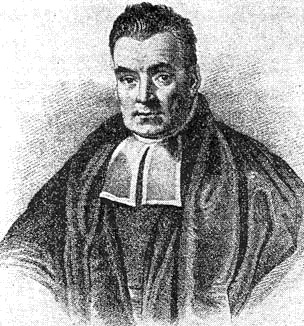
\includegraphics[scale=0.6]{figures/Thomas_Bayes.jpeg}
    \caption{Thomas Joshua Bayes (1702-1761)}
    \label{fig:my_label2}
\end{figure}



Seu trabalho com as probabilidades foi reunido em um ensaio
publicado após a sua morte (em 1763) no livro Philosophical
Transactions of the Royal Society of London. O ensaio Essay
Towards Solving a Problem in the Doctrine of Chances relatou,
entre outras importantes descobertas de Bayes, o famoso Teorema de
Bayes.

\subsection{ O Que é o Teorema de Bayes}

O teoréma de Bayes é usado na inferência estatística para
atualizar estimativas da probabilidade de que diferentes hipóteses
sejam verdadeiras, baseado nas observações e no conhecimento de
como essas observações se relacionam com as hipóteses.\vskip0.3cm

Este teorema é uma das pedras angulares da estatística das
probabilidades combinadas, e é largamente utilizada em áreas a
primeira vista pouco relacionadas, como Medicina e
Informática.\vskip0.3cm

Na primeira, o paradigma embasado em evidências é todo construído
em cima do teorema de Bayes. Baseado na experiência acumulada de
exames e testes para tentar diagnosticar uma doença, o médico
enquadra seus pacientes e pode estimar qual a probabilidade de que
uma dada doença esteja se manifestando. Ou seja, dada uma
probabilidade inicial (por exemplo, o paciente é fumante) e
aplicado um exame em que, se sabe, há uma probabilidade de
falsos-positivos e falso-negativos (por exemplo, uma biópsia de
pulmão), o médico sabe qual a probabilidade resultante daquele
paciente ter a doença (por exemplo, câncer de pulmão).\vskip0.3cm

Na informática, muitos dos sistemas de classificação automática
são baseados no teorema de Bayes. Inicialmente o sistema é
treinado, aceitando entradas de humanos que dizem que uma dada
entrada pertencem a determinado grupo. Com o tempo, o sistema
acumula um grande banco dessas informações e, aplicando o teorema
de Bayes, consegue estimar a probabilidade de cada novo dado de
pertencer a cada grupo já classificado.\vskip0.3cm


\subsection{Definição}

Seja $B_{1},B_{2},...,B_{k}$ uma partição do espaço amostral S e
seja A um evento associado a S. aplicando-se a definição de
probabilidade condicionada, poderemos escrever


\begin{equation}\label{bayes}
    P(B_{i}/A)=\frac{P(A/B_{i})P(B_{i})}{\sum_{j=1}^{k}P(A/B_{j})P(B_{j})}
\end{equation}


Esse resultado é conhecido como \emph{Teorema de Bayes}. È também
denominado fórmula da probabilidade das causas (ou dos
antededentes). Desde que os $B_{i}$ constituam uma partição do
espaço amostral um, e somente um, dos eventos $B_{i}$ ocorrerá.

\newpage
\section{Eventos Independentes}

Já consideramos eventos A e B que não podem ocorrer conjuntamente,
isto é, $A\cap B = \phi$. Tais eventos são denominados mutuamente
excludentes, ou eventos incompatíveis. Observamos anteriormente
que se A e B forem mutuamente excludentes, então $PA/B=0$, porque
a ocorrência dada de B impede a ocorrência de A. No outro extremo,
temos a situação já estudada, na qual $B \supset A$ e,
consequentemente, $P(B/A)=1$.\vskip0.3cm

Consideremos $P(A \cap B)$, supondo que as probabilidades
condicionadas sejam iguais às correspondentes probabilidades
absolutas. Teremos:

$$
P(A \cap B)= P(A/B)P(B)=P(A)P(B)
$$

$$
P(A \cap B)= P(B/A)P(A)=P(B)P(A)
$$


Desse modo, desde que nem P(A) nem P(B) sejam iguais a zero,
verificamos que as probabilidades absolutas serão iguais às
probabilidades condicionais se, e somente se, $P(A \cap
B)=P(A)P(B)$. Em consequência, formulamos a seguinte definição, a
qual será também válida quer P(A) ou P(B) seja nulo:\vskip0.3cm

\textbf{Definição:} A e B serão eventos independentes se, e
somente se,

$$
P(A \cap B) = P(A)P(B)
$$


Será importante para nós, estendermos a noção de independência
para mais de dois eventos. Consideremos, inicialmente, três
eventos associados a um experimento, digamos A, B e C. Se A e B, A
e C, B e C forem independentes dois a dois (no sentido acima),
então não se concluirá, em geral, que não exista dependência entre
os três eventos.\vskip0.3cm

\textbf{Definição:} Diremos que os três eventos A, B e C são
mutuamente independentes se, e somente se, todas as condições
seguintes forem válidas:

$$
P(A \cap B)=P(A)P(B)
$$

$$
P(A \cap C)=P(A)P(C)
$$

$$
P(B \cap C)=P(B)P(C)
$$

$$
P(A \cap B \cap C)=P(A)P(B)P(C)
$$


Finalmente, generalizando esta noção para n eventos, na seguinte
definição:\vskip0.3cm



\textbf{Definição:} Os n eventos $A_{1},A_{2},...,A_{n}$ serão
mutuamente independentes se, e somente se, tivermos para
$k=2,3,...,n$:

\begin{equation}\label{}
    P(A_{i_{1}} \cap A_{i_{2}} \cap A_{i_{k}})=
    P(A_{i_{1}})P(A_{i_{2}})...P(A_{i_{k}})
\end{equation}



\newpage
\section{Principais Distribuições de Probabilidade}
 
 
\inic Uma distribuição de probabilidade é um modelo matemático que relaciona um certo valor da variável aleatória em estudo com a sua probabilidade de ocorrência. De conformidade com a natureza da variável aleatória, a distribuição pode ser classificada em discreta ou contínua.
 
\subsection{Distribuição Binomial}

Os princípios básicos da distribuição binomial foram desenvolvidos pelo matemático suíço durante o século XVII chamado \textbf{Jakob Bernoulli}, que fez muitas contribuições à teoria da probabilidade. Foi o autor do que é geralmente conhecido como o primeiro livro dedicado à probabilidade, publicado em 1713.


\begin{figure}
    \centering
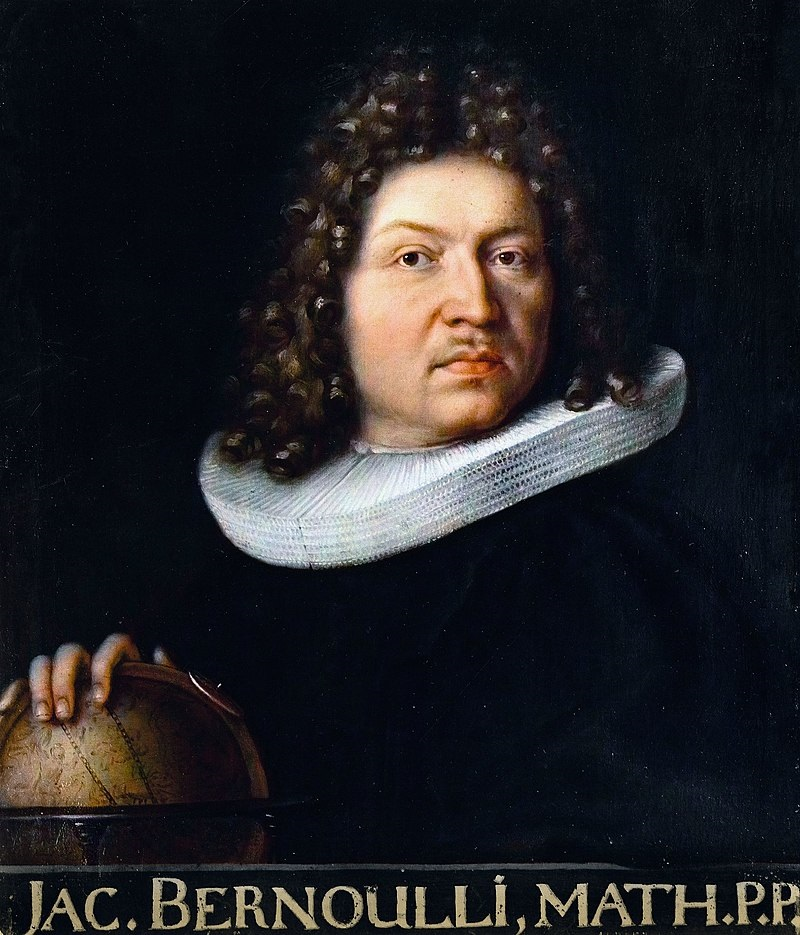
\includegraphics[scale=0.2]{figures/Jakob_Bernoulli.jpeg}
    \caption{Jakob Bernoulli(1654-1705)}
    \label{fig:my_label4}
\end{figure}

Jakob nasceu em Basel na Suiça, estudou Teologia, Matemática e Astronomia na Universidade de Basel. Entre os nomes associados à instituição estão os de \textbf{Leonhard Euler}, \textbf{Friedrich Nietzsche}, e \textbf{Eugen Huber} um jurista famoso e criador do Código Civil Suiço. \vskip0.3cm

Em homenagem a Jakob, os ensaios utilizando probabilidade binomial, na maioria das vezes são denominados \textbf{Ensaios de Bernoulli}, e uma sequência desse tipo de ensaios é denominado de \textbf{Processo de Bernoulli} \vskip0.3cm


A distribuição Binomial dá a probabilidade de deterninado desfecho ocorrer em determinado número de ensaios independentes. \vskip0.3cm


\inic A distribuição Binomial é uma distribuição discreta, cuja função de probabilidade é:
 
\begin{equation}
f(y) = C_{n}^{y}p^{y}q^{n-y}
\end{equation}
 
Sendo: \vskip0.3cm

\begin{itemize}
\item $p$ = probabilidade de realização do acontecimento favorável; 
\item  $q$ = probabilidade de ralização do acontecimento contrário;  
\item $y$ = número de vezes que se realiza o acontecimento favorável;  
\item $n$ = número de tentativas; 
\item $C_{n}^{y}$ = números de combinações de n elementos, tomados y a y; 
\end{itemize} 

\newpage
\subsection{Distribuição de Poisson}

A distribuição de Poisson tem este nome em homenagem ao metemático, Astrônomo e físico francês \textbf{Simeon Denis Poisson}. Com característica próxima a Binomial, a distribuição de Poisson é uma distribuição descontínua, aplicável quando o resultado é o número de vezes que determinado evento ocorre. 

\begin{figure}
    \centering
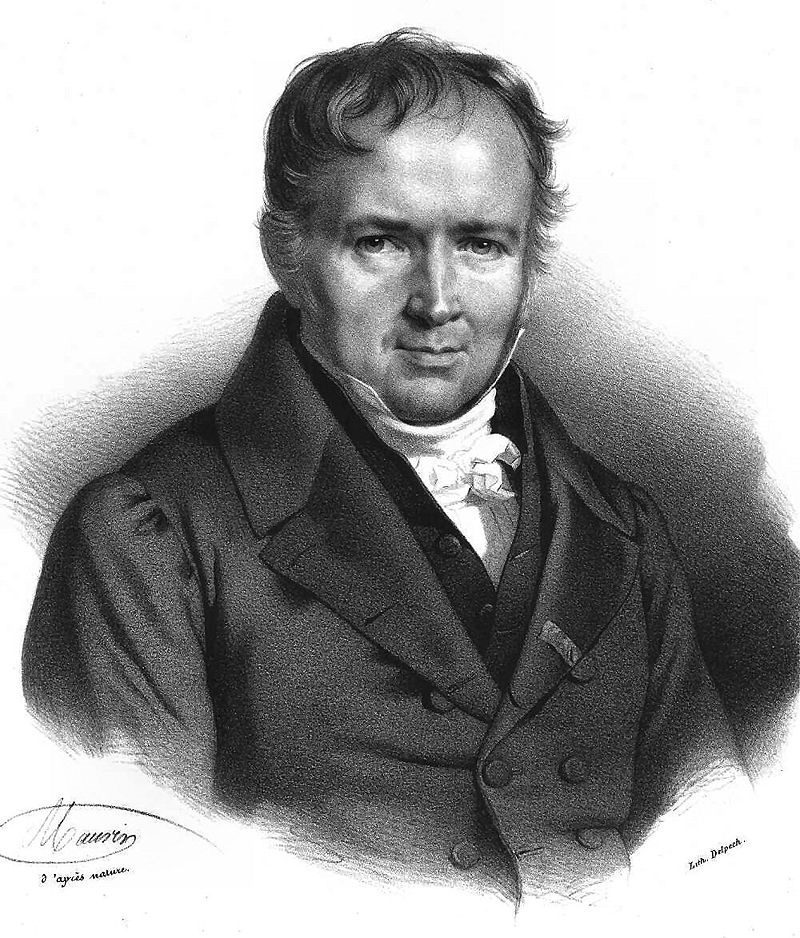
\includegraphics[scale=0.2]{figures/Simeon_Poisson.jpeg}
    \caption{Simeon Denis Poisson(1781-1840)}
    \label{fig:my_label4}
\end{figure}


Poisson recebeu dois prêmios importantes da época:

\begin{itemize}
    \item \textbf{Prêmio Lalande} (1810) Membro da Academia Americana de Artes e Ciências;
    \item \textbf{Medalha Copley} (For his work entitled, Nouvelle Theorie de lAction Capillaire., 1832)
\end{itemize}

O Prêmio Lalande foi uma condecoração científica em Astronomia, concedida de 1902 a 1970 pela Académie des Sciences. O prêmio homenageia o astrônomo Jérôme Lalande, estabelecido pelo próprio em 1801. Após 1970 foi combinado com o prêmio da fundação Benjamin Valz, concedido até 1996.\vskip0.3cm


A Medalha Copley é um prêmio no domínio das ciências, sendo
a de maior prestígio atribuída pela \textbf{Royal Society} e, também, a mais antiga. Foi concedida pela primeira vez em 1731.\vskip0.3cm


  
\inic A distribuição de Poisson é adequada para descrever as probabilidades do número de ocorrências num intervalo contínuo (em geral tempo ou espaço). São exemplos de variáveis que podem ter como modelo a distribuição de Poisson:

\begin{enumerate}
    \item Acidentes com automóveis em uma determinada estrada;
    \item Quantidade de pacientes que chegam num pronto socorro durante a madrugada;
    \item  Número de leitos necessários em centro de tratamento intensivo;
    \item  Número de Policiais Militares ou Agentes de Trânsito, necessários em um quadro de distribuição de modo a assegurar a disponibilidade de recursos adequados;
\end{enumerate}



\inic Note que a quantidade de valores possíveis que a variável aleatória pode assumir é infinita, entretanto enumerável. Além disso, observe que a variável aleatória é discreta (número de ocorrências), no entanto a unidade de medida é contínua (tempo, área).\vskip0.3cm

Ainda, as falhas não são contáveis. Por exemplo, não é possível contar os acidentes que não ocorreram em um dia, nem tão pouco a quantidade de pacientes que não chegaram ao pronto socorro na madrugada.
 
 
\begin{equation}
    P\left(X=k\right)= \frac{e^{-\lambda}\lambda^{k}}{k!}
\end{equation}

onde:

\begin{itemize}
\item $e$: é a base do logaritmo natural ou neperiano;
\item $k$: quantidade de ocorrências num intervalo contínuo;
\item $k!$: é o fatorial de $k$; 
\item $\lambda$: é um número real que representa a taxa de ocorrência. Por exemplo, se o evento ocorre a uma média de 4 minutos e estamos interessados no número de eventos que ocorrem num intervalo de 10 minutos, $\lambda={10}/{4}=2.5$
\end{itemize}

  
Além disso, temos que o valor esperado e a variância serão: 

$$
\begin{aligned}
E\left[X\right] =\lambda \\
Var\left(X\right) = \lambda
\end{aligned}
$$
 



\subsection{Distribuição Normal}

Para alguns autores, a distribuição de probabilidade mais famosa da estatística, é denominada \textbf{Distribuição Normal}, \textbf{Curva de Gauss}, \textbf{Gaussiana}, \textbf{Distribuição de Laplace–Gauss} ou em \textbf{Forma de Sino}.\vskip0.3cm 


A curva foi descoberta pela primeira vez pelo matemático francês \textbf{Abraham de Moivre} e publicada em 1733. No entanto, dois matemáticos, o francês \textbf{Pierre-Simon Laplace} em 1777 e o alemão \textbf{Karl Friedrich Gauss} em 1809, foram responsáveis pelo estabelecimento dos princípios científicos da distribuição normal.\vskip0.3cm 

\begin{figure}
    \centering
    \caption{Abraham de Moivre(1667-1754)} 
    \centering
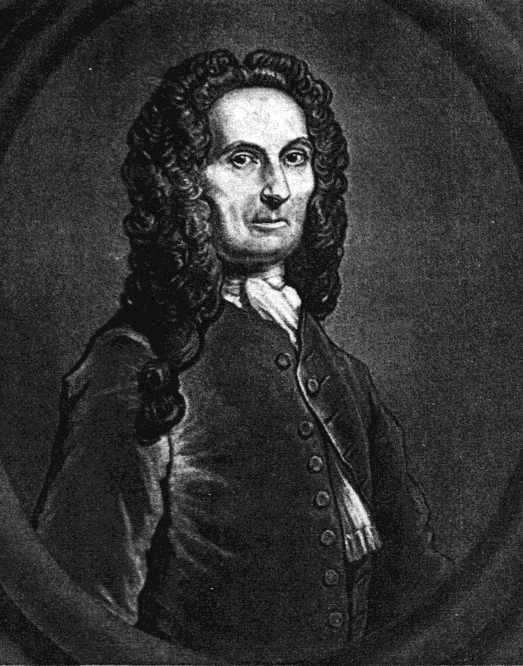
\includegraphics[scale=0.2]{figures/Abraham_de_moivre.jpeg}
%\legend{Fonte: Wikimedia Foundation, 2022.}
    \label{fig:my_label6} 
\end{figure}

%ABRAHAM DE MOIVRE. In: WIKIPÉDIA, a enciclopédia livre. Flórida: Wikimedia Foundation, 2022. Disponível em: <https://pt.wikipedia.org/w/index.php?title=Abraham_de_Moivre&oldid=64507244>. Acesso em: 4 out. 2022.

Diversos autores consideram Laplace como tendo realizado as maiores contribuição à teoria da probabilidade, mas foi dado o nome de Gauss para a distribuição depois de ele tê-la aplicado a teoria dos movimentos dos corpos celestes.\vskip0.3cm 


\inic Quando os valores das observações de uma variável resposta, originados de uma amostra, são agrupados em tabelas de frequências, objetiva-se conhecer a variação e como se processa a distribuição dos dados.\vskip0.3cm 

\inic Existem inúmeros tipos de curvas que podem representar as distribuições. Na maioria das pesquisas na Gestão Pública, as observações variam em torno da distribuição normal, a qual é uma distribuição contínua. É a mais importante distribuição no campo da Estatística e tem a seguinte função de densidade:\vskip0.3cm 


\begin{equation}
f\left(x\right) = \frac{1}{\sqrt{2\pi \sigma^2}}exp \left\{-\frac{1}{2}\left(\frac{x-\mu}{\sigma}\right)^2 \right\},~~~-\infty<x<\infty~~\text{e}~\sigma>0
 \end{equation} 

È uma curva estável, em forma de sino, e simétrica em torno da média da distribuição, simbolizada pela letra grega mi. O desvi0-padrão da distribuição é simbolizado pela letra grega sigma.\vskip0.3cm 















\newpage
\subsection{Distribuição $t$ de $Student$}
\subsubsection{A Origem da $t$ $student$}

William Sealy Gosset nasceu em 13 de junho de 1876 em Canterbury, Inglaterra, o primeiro de cinco filhos do Coronel Frederic Gosset e Agnes Sealy Vidal. Ele tinha problemas de visão e não conseguia seguir seu pai na Royal Engineers, mas ele era um aluno muito bom e ganhou várias bolsas de estudo.

\begin{figure}
    \centering
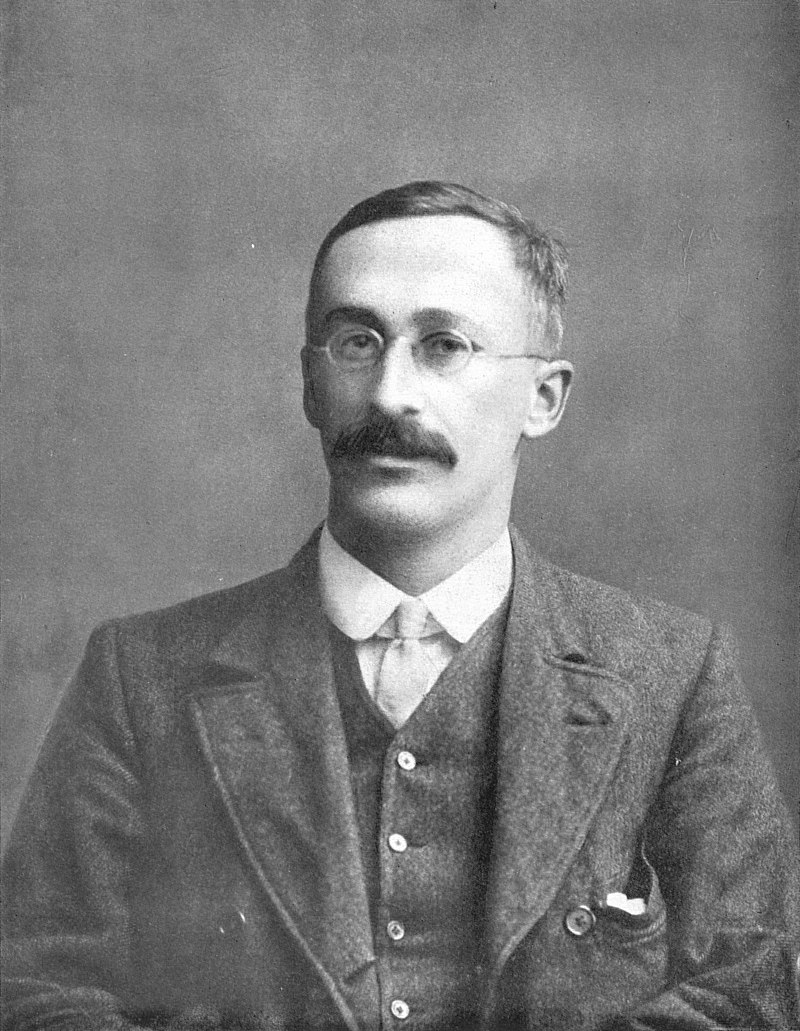
\includegraphics[scale=0.15]{figures/William_Sealy_Gosset.jpeg}
    \caption{William Sealy Gosset(1876-1937)}
    \label{fig:my_label3}
\end{figure}


Ao final do século XIX, a famosa \textbf{Arthur Guinness Son and Company} era a maior cervejaria do mundo, e foi pioneira em diversos esforços para o Controle de Qualidade. Em 1899, um dos contratados para o cargo de químico, recém-formado na Universidade de Oxford, com 23 anos de idade e um currículo que combinava matemática e estatística, foi \textbf{William Sealy Gosset}.\vskip0.3cm

%\begin{figure}[!htb]
%\centering{
% 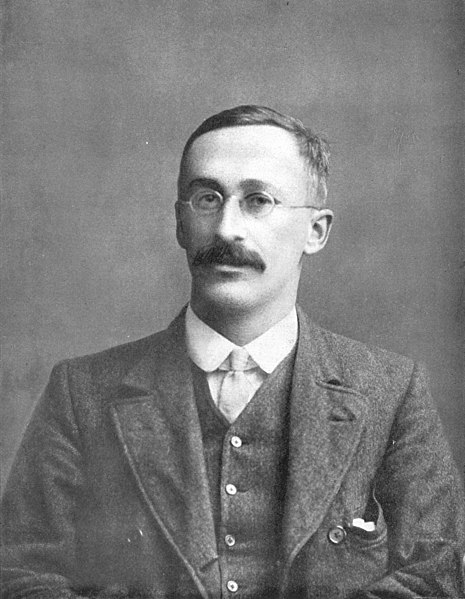
\includegraphics[scale=0.5]{figures/Gosset2.png}\\
%  \vspace{-0.8cm}
%  \caption{William Sealy Gosset, 1908}\label{esquematabela1}}
%\end{figure}


A Guinness era uma empresa de Agro-Química progressista e Gosset iria aplicar os seus conhecimentos de estatística tanto na cervejaria (a destilaria) como nas quintas, para a selecção dos melhores espécimens de cevada.\vskip0.3cm

O trabalho de Gosset na Guinness consistia em medir os inúmeros fatores do processo de produção e ponderar como eles se relacionam aos resultados do produto final. William realizou muitos testes para estimar a duração da cerveja diante das diferentes condições de armazenagem, fabricação e transporte.\vskip0.3cm


Gosset desenvolveu o teste t, distribuição passível de ser tabulada, como um modo barato de monitorar a qualidade da cerveja. Na época, não existia uma teoria para a tomada de decisões com base em pequenas amostras. Por isso, o grande diferencial desse teste é justamente permitir que se façam inferências usando um menor número de elementos. \vskip0.3cm

Um outro funcionário da Guinness tinha já publicado um trabalho que continha alguns segredos da Cervejeira Guinness. Para prevenir fugas de informação e futuras revelações dos "segredos" da marca, a Guinness proibiu que os seus empregados pudessem publicar quaisquer trabalhos independentemente do conteúdo. Isto queria dizer que Gosset não tinha como publicar os trabalhos com o seu nome. Então, usou o pseudonimo $Student$ para as suas publicações evitando ser detectado pela entidade empregadora. \vskip0.3cm

Desta forma, o seu feito mais conhecido, é hoje conhecido com a Distribuição t-Student, que noutras circunstâncias seria conhecida como a Distribuição t-Gosset.\vskip0.3cm


Gosset trabalhou na cervejaria em St. James's Gate por 36 anos, antes de se tornar o cervejeiro-chefe de uma nova cervejaria Guinness em Park Royal em Londres.\vskip0.3cm

Em outubro de 2012, uma placa foi inaugurada na Escola Nacional de St Patrick, Blackrock(Irlanda), para homenagear William Sealy Gosset, que morou nas proximidades por 22 anos. \vskip0.3cm

Sir \textbf{Ronald Fisher}, um gigante entre os estatísticos, chamou Gosset de “O Faraday das Estatísticas”, reconhecendo sua capacidade de compreender princípios gerais e aplicá-los a problemas de importância prática.



\subsubsection{A Distribuição $t$ }

Seja a variável aleatória:

\begin{equation}
    t =\frac{\overline{y}-\overline{Y}}{\frac{s(Y)}{\sqrt(n)}}
\end{equation}

Esta variável é conhecida com distribuição $t$ student, com $k=n-1$ graus de liberdade, podendo também ser escrita na forma:

\begin{equation}
    t =\frac{N(0,1)}{\sqrt{\frac{\chi^{2}_{n-1}}{n-1}}}
\end{equation}

O $s(y)$ é considerado o desvio-padrão estimado.\vskip0.3cm

O gráfico da função densidade da variável $t$ de student é simétrico e tem uma forma parecida com a distribuição normal, entretando, menos achatada, com a média zero e variância igual $\frac{k}{(k-2)}$, em que $k>2$ graus de liberdade. A função densidade da variável $t$ é dada pela expressão (2.10). 

\begin{equation}
f\left(t\right)=\frac{1}{\sqrt{k \pi}}\frac{\Gamma\left(\frac{k+1}{2}\right) }{\Gamma \left(\frac{k}{2}\right)}\left(1+\frac{t^2}{k}\right)^{-\left(\frac{\upsilon+1}{2}\right)},~~~-\infty<x<\infty
\end{equation}





















 